\section{The Mandelbrot set using OpenMP}
For the Mandelbrot using OpenMp we base our strong scale analysis on the closely related speedup and efficiency plot in Figure \ref{fig:mandel}. For reference the dotted curves represent in both plots theoretical optimum. The first point that stands out is that the speedup and the efficiency does not depend on the resolution.
This suggests that when increase the resolution the proportion of workload remains the same.
Looking at the observed speedup, from single to 2 threads the speedup almost ideal, but from 2 to 4 threads the speedup stays almost identical, following that, the speedup increases steadily.
A key observation is that for higher number of threads the speedup moves farther away from the ideal curve due to increased costs, such as synchronization time, memory bandwidth limitations and cache contention.
This behavior can directly translated to the efficiency plot as well, where the efficiency decreases quickly and then deceases at a lower rate until from 16 to 20 threads the efficiency is almost identical.
This is a common behavior in strong scaling experiments, because at a certain point the same factor as mentioned in the speedup plot start to weigh in and slow the implementation down, particularly with a higher number of threads.
\begin{table}[H]
\centering
\begin{tabular}{|c|c|c|c|}
\hline
\textbf{Threads} & \textbf{Iterations/second} & \textbf{MFlop/s:} & \textbf{Total time:} \\ \hline
1                & 2.075e+08                  & 1660.67           & 155.782              \\
2                & 4.144e+08                  & 3315.96           & 78.036               \\
4                & 4.291e+08                  & 3433.23           & 75.370               \\
8                & 6.393e+08                  & 5115.16           & 50.587               \\
16               & 1.130e+09                  & 9045.01           & 28.608               \\
20               & 1.397e+09                  & 11177.4           & 23.150               \\ \hline
\end{tabular}
\caption{Subset of benchmark key values for the resolution 4096 $\times$ 4096 with roughly 32.34 billion iterations}
\label{tab:mandel-bench}
\end{table}
The benchmarking used in this exercise also evaluates other fascinating key values, in Table \ref{tab:mandel-bench} we can see an example for a specific resolution, where we can clearly see that when increasing the number of threads more iterations per second can be executed, which is also reflected in the MFlop/s and the decreasing total execution time. This shows the effective distribution of the workloads across multiple threads, but the gains made by adding more threads, as seen in the efficiency and speedup plot, will at some point have diminishing returns. 
Overall the performance gains are significant, especially up to 16 threads.
\begin{figure}[H]
    \centering
        \centering
        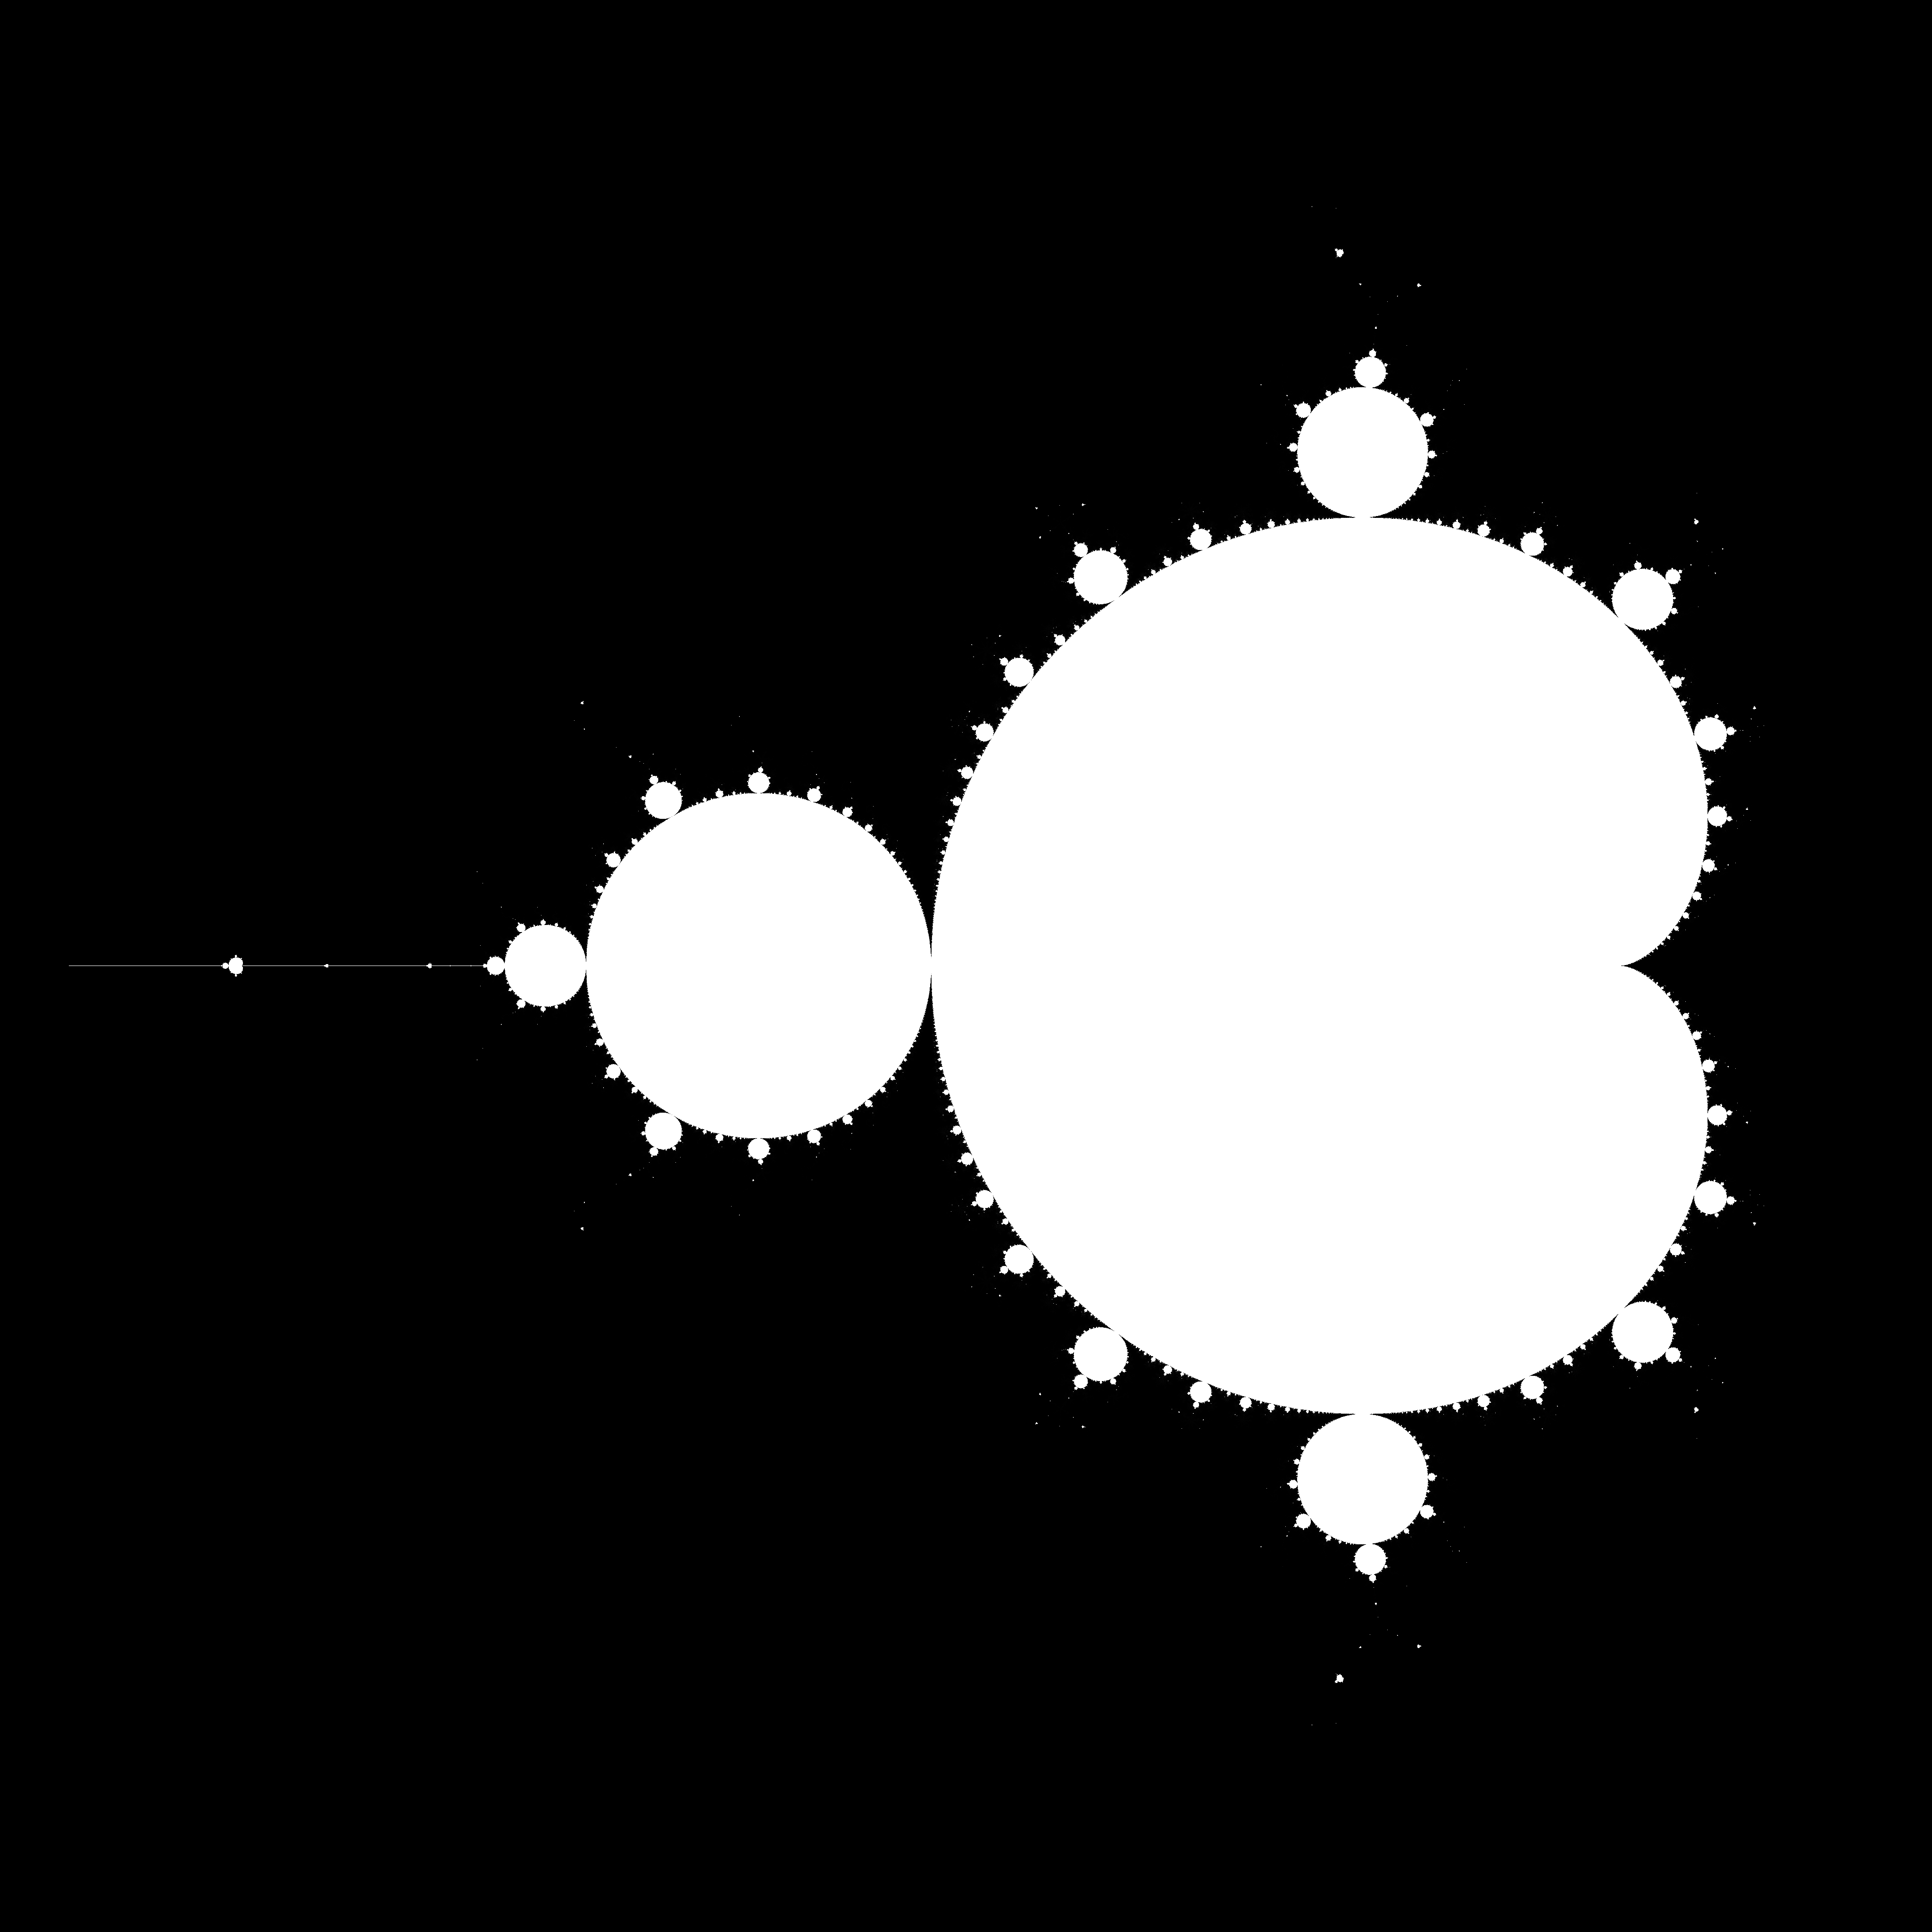
\includegraphics[width=0.4\textwidth]{../media/mandel_parallel.png}
        \caption{The Mandelbrot set with resolution 4096 $\times$ 4096 using parallel OpenMP implementation}
        \label{fig:mandel_imaage}
    \end{figure}
Also important to mention is that in my implementation, I use \texttt{omp for collapse(2)} statement, in order to parallelize over both outer loops, which iterate over the x and y coordinates. I used this with the premise to allow multiple loops to be collapsed into a single loop and parallelize them a single entity, hence trying to have the iteration space evenly spread out over all processes. Comparing my results with two of my fellow students, which use a standard \texttt{omp for} loop, showed no significant improved or deterioration in execution time. This leads me to believe that OpenMP performs very similar optimization based on both statements.
\begin{figure}[H]
    \centering
    \begin{subfigure}[b]{\textwidth}
        \centering
        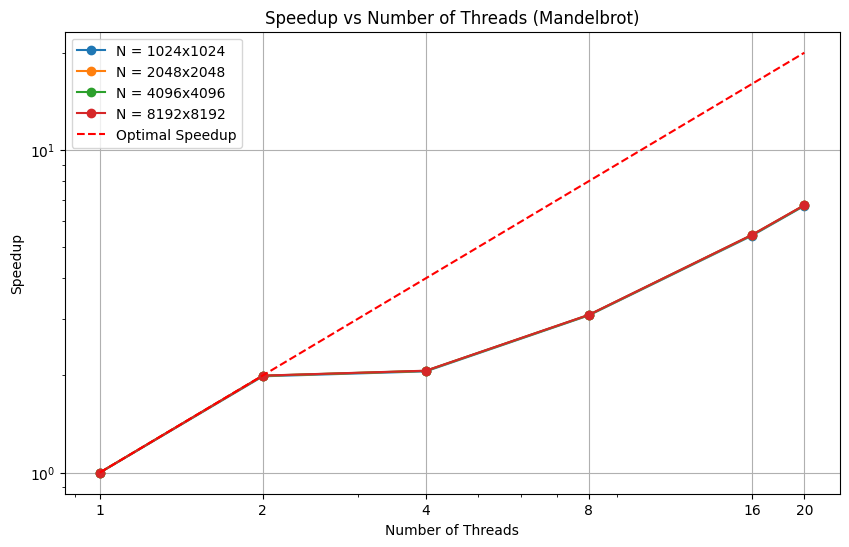
\includegraphics[width=\textwidth]{../media/mandel_speedup.png}
        \caption{Speedup}
        \label{fig:image1}
    \end{subfigure}
    \hfill \\
    \begin{subfigure}[b]{\textwidth}
        \centering
        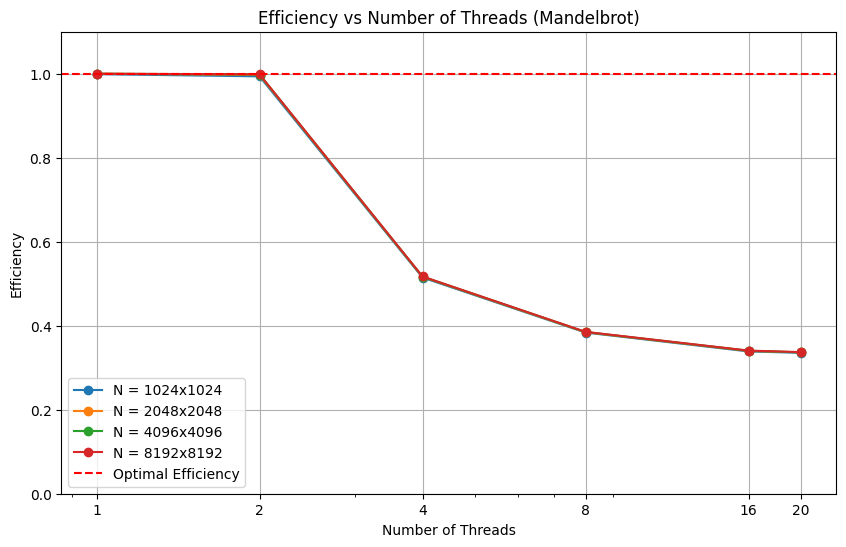
\includegraphics[width=\textwidth]{../media/mandel_eff.png}
        \caption{Efficiency}
        \label{fig:image2}
    \end{subfigure}
    \caption{Speedup and Efficiency for the Mandelbrot implementation}
    \label{fig:mandel}
\end{figure}


 

